\documentclass[a4paper,titlepage]{book}
\usepackage{graphicx}
%\usepackage{c:/home/wpenny/software/latex-graphics/graphicx.sty}

\newcommand{\bi}{\begin{itemize}}
\newcommand{\ei}{\end{itemize}}

\begin{document}

\chapter{Face fMRI data}

As a third and more sophisticated example, consider the data from a repetition priming experiment performed using event-related fMRI. Briefly, this is a 2x2 factorial study with factors `fame' and `repetition' where famous and non-famous faces were presented twice against a checkerboard baseline. The subject was asked to make fame judgements by making key presses. There are thus four event-types of interest; first and second presentations of famous and non-famous faces, which 
we denote N1, N2, F1 and F2. The experimental design is shown shematically in Figure~\ref{face_design}.
\begin{figure}
\begin{center}
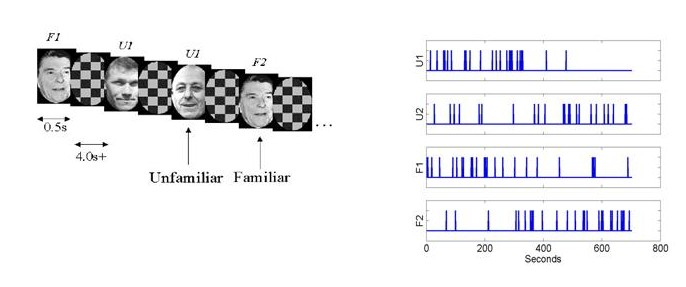
\includegraphics[width=150mm]{face_paradigm}
\caption{\em Face repetition paradigm. {\bf Left} There were 2 presentations of 26 Famous and 26 Nonfamous Greyscale photographs, for 0.5s each, randomly intermixed. The 
minimal Stimulus Onset Asynchrony (SOA)=4.5s, with probability 2/3 (ie 1/3 null events). The subject made one of two 
right finger key presses denoting whether or not the subject thought the face was famous. {\bf Right} The time series of events. \label{face_design}}
\end{center}
\end{figure}


Images were acquired using continuous Echo-Planar 
Imaging (EPI) with TE=40ms, TR=2s and 24 descending slices (64x64 3x3$mm^2$), 3mm thick with a 1.5mm gap.
The data archive is available from 
This contains 351 Analyse format functional images
\verb!sM03953_0005_*.img! of dimension 
64x64x24 with 3mmx3mmx4.5mm voxels. A strucural 
image is also provided \verb!sM03953_0007.img! also in Analyse format.

To analyse the data, first create a new directory DIR 
\newline \verb!eg. c:\home\wpenny\fmri_analysis\face-rep\all!, in which to place the results
of your analysis. Then create 3 subdirectories (i) \verb!jobs!, 
(ii) \verb!designs!, (iii) \verb!classical! and (iv) \verb!bayesian!. As the analysis 
proceeds these directories will be filled with job-specification files, design matrices 
and models estimated using classical or Bayesian 
methods. Additionally, in each of the \verb!designs!, \verb!classical! and \verb!bayesian! directories create 
two subdirectories called \verb!categorical! and 
\verb!parametric! as we will show how this data 
can be analysed in two different ways. 
In the categoral analysis we will look at the 
main effects of fame and repetition and in the 
parameteric analysis we will look at 
responses as a function of `lag', that is, the number of faces intervening between repetition of a specific face.

Start up matlab, enter your jobs directory and type {\em spm fmri} at the matlab prompt. SPM will then open in fMRI mode with three windows (1) the top-left or `command' window, (2) the 
bottom-left or `interactive' window
and (3) the right-hand or `graphics' window. 
Analysis 
then takes place in three major stages (i) 
spatial pre-processing, (ii) model specification, review 
and estimation and (iii) inference. These stages organise the buttons 
in SPM's base window.
\begin{figure}
\begin{center}
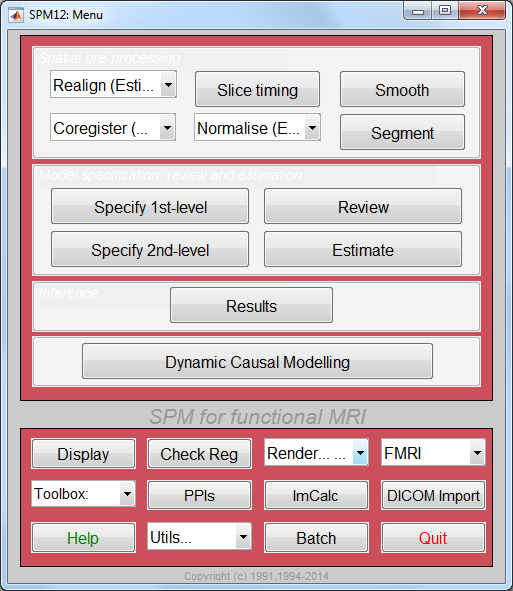
\includegraphics[width=100mm]{command}
\caption{\em The SPM base window comprises 
three sections i) 
spatial pre-processing, (ii) model specification, review 
and estimation and (iii) inference. \label{command}}
\end{center}
\end{figure}

\section{Spatial pre-processing}

\subsection{Display}

Display eg. the first functional image using the 
`Display' button. Note orbitofrontal 
  and inferior temporal drop-out and ghosting. This 
  can be seen more clearly by selecting `brighten if necessary' from the `Effects' tab at the top of the 
  graphics window.
  \begin{figure}
\begin{center}
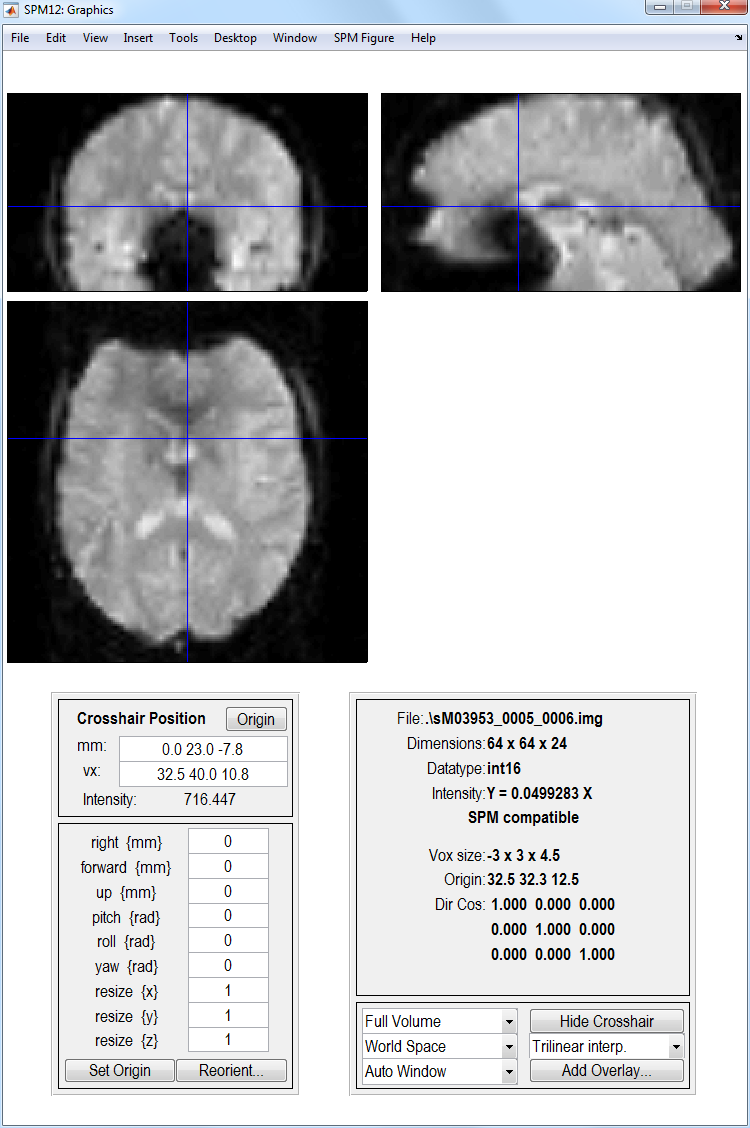
\includegraphics[width=100mm]{dropout}
\caption{\em Signal dropout in EPI images. \label{dropout}}
\end{center}
\end{figure}

\subsection{Realignment}

Under the spatial pre-processing section of the SPM base window select `Realign' from the `Realign' pulldown menu. This will call up a realignment job specification 
in the graphics window.
Then
\bi
\item{Select `New Realign:Estimate and Reslice'}
\item{Open the newly created `Realign:Estimate and Reslice' option.}
\item{Highlight data, select `New Session', then highlight the newly created `Session' option.} 
\item{Select `Specify Files' and use the SPM file selector
to choose all of your functional images eg. \verb!sM03953_0005_*.img!.}
\item{Save the job file as eg. {\sf DIR/jobs/realign.mat}}.
\item{Press the RUN button in the graphics window.}
\ei
This 
will run the realign job which will write realigned images into the directory where the functional images
are. These new images will be prefixed with the letter `r'. SPM will then plot the estimated time series of translations and rotations shown in Figure~\ref{face_realign}. These data, the realignment parameters, are also saved to 
a file eg. \verb!rp_sM03953_0005_0006.txt!, so that these variables can be used as regressors when fitting GLMs. To prepare for this copy the file into the 
\verb!DIR\jobs\! directory and rename it \verb!movepars.txt!.
This allows movements effects to be discounted when
looking for brain activations.

SPM will also create a mean image eg. 
\verb!meansM03953_0005_0006.img! which will be used in the next
step of spatial processing - coregistration.
\begin{figure}
\begin{center}
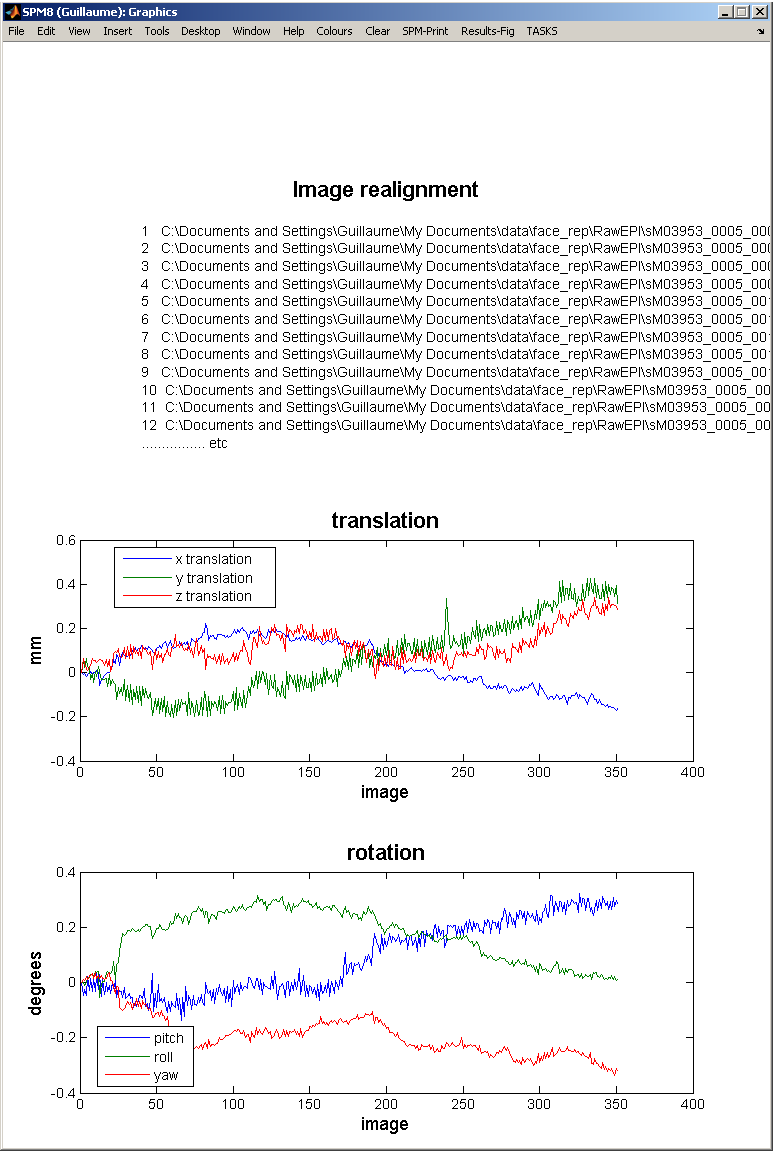
\includegraphics[width=100mm]{realign}
\caption{\em Realignment of face data.\label{face_realign}}
\end{center}
\end{figure}

\subsection{Slice timing correction}

Press the `Slice timing' button. This will call up the specification of a slice timing job in the graphics 
window. 
\bi
\item{Open the `Slice Timing' option}
\item{Highlight `Data' and select `New Sessions'}
\item{Highlight the newly create `Sessions' option, `Specify Files' and select the
351 realigned functional images using the 
filter \verb!^r.*!.}}
\item{Select `Number of Slices' and enter 24}
\item{Select TR and enter 2}
\item{Select TA and enter 2}
\item{Select `Slice order' and enter 24:-1:1}
\item{Select `Reference Slice', and enter 12}
\item{Save the job as \verb!slice_timing.mat! and press `Run'}
\ei
SPM will write slice-time corrected files with 
the prefix `a' in the functional data directory.

\subsection{Coregistration}

Press the `Coreg' button. This will call up the specification of a coregistration job in the graphics 
window. 

\bi
\item{Select New "Coreg:Estimate"}
\item{Double-click on the newly created Coreg:Estimate}
\item{Highlight `Reference Image' and then select the
 mean functional image
\verb!meansM03953_0005_0006.img!}
\item{Highlight `Source Image' and then select 
the structural image eg. \verb!sM03953_0007.img!.}
\item{Press the Save button and save the job as 
{\sf coreg.job}}
\item{Then press RUN}
\ei
SPM will then implement a coregistration between the structural and functional data that maximises the mutual information. The image in figure~\ref{aud_coreg} should then appear 
in the graphics window. SPM will have changed the header 
of the source file which in this case is the 
structural image \verb!sM03953_0007.img!.
\begin{figure}
\begin{center}
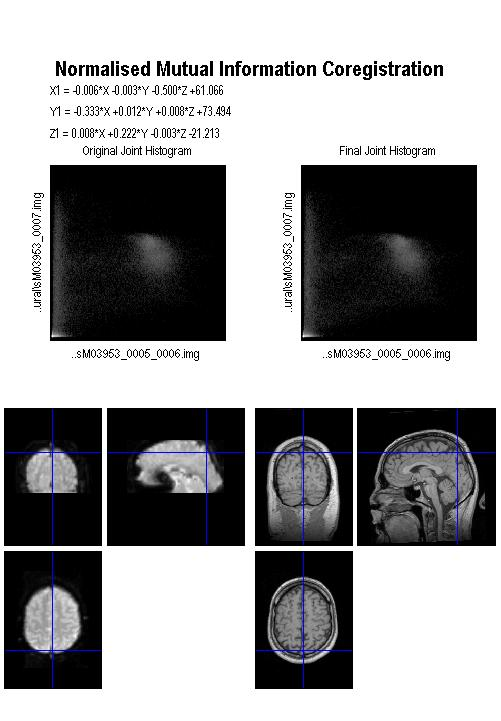
\includegraphics[width=100mm]{coreg}
\caption{\em Mutual Information Coeregistration  of Auditory data. \label{aud_coreg}}
\end{center}
\end{figure}

\subsection{Segmentation}

Press the `Segment' button. This will call up the specification of a segmentation job in the graphics 
window. Highlight the Data field and then select 
the subjects coregistered anatomical image 
eg. \verb!sM03953_0007.img!. Save the job file
as {\sf segment.mat} and then press RUN.
SPM will segment the structural image using 
the default tissue probability maps as 
priors. 
SPM will create, by default, gray and white matter
images and bias-field corrected structral image.
These can be viewed using the CheckReg facility 
as described in the previous section (press segement 
and select . Figure \ref{aud_gray} shows the gray matter image, \verb!c1sM03953_0007.img! along with the original structural.
\begin{figure}
\begin{center}
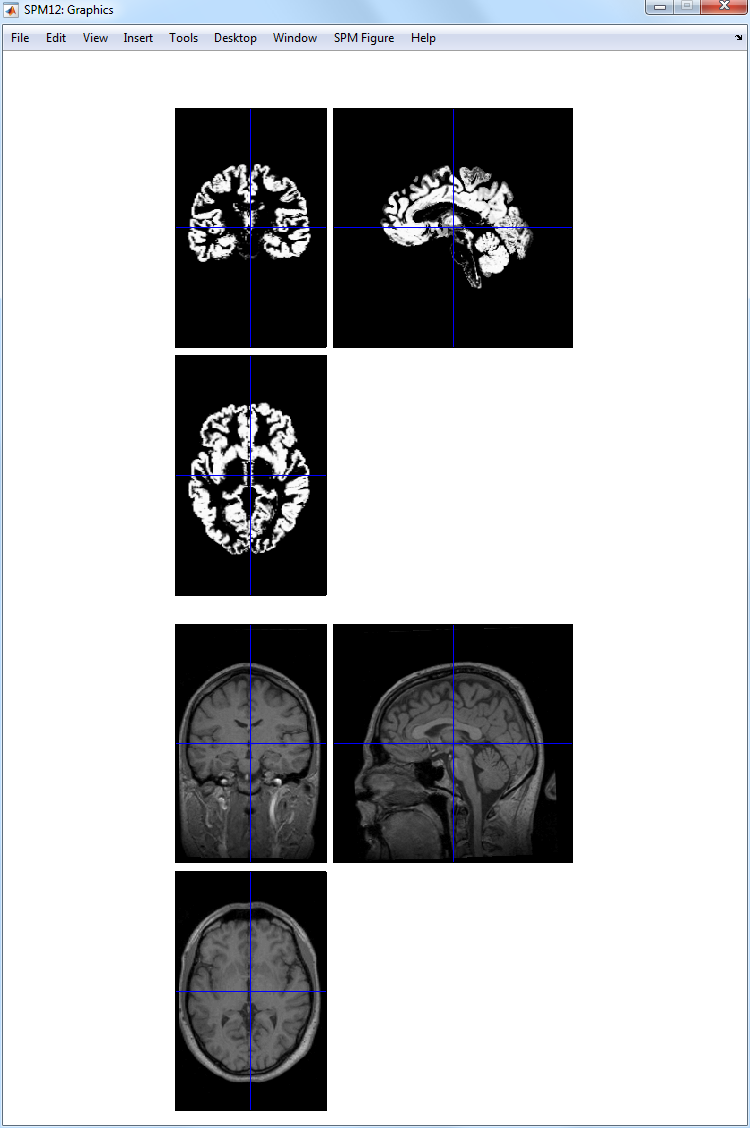
\includegraphics[width=100mm]{gray}
\caption{\em Gray matter image and `registered' structural image. \label{face_gray}}
\end{center}
\end{figure}

SPM will also write a spatial normalisation eg. 
\verb!sM03952_0007_seg_sn.mat! file in the 
original structural directory. This will be used 
in the next section to normalise the functional data. 


\subsection{Normalize}

Press the `Normalize' button. This will call up the specification of a normalise job in the graphics 
window. 

\bi
\item{Select a New "Normalise:Write" field. This 
allows previously estimated warps to be applied to 
a series of images.}
\item{Highlight `Data', select New "Subject"}
\item{Open `Subject', highlight `Parameter File' and 
select the \verb!sM03952_0007_seg_sn.mat! file that you 
created in the previous section}
\item{Highlight images to write and select all of the 
slice-time corrected, realigned functional images `arsM*.img'. Note: This can be done efficiently by changing the filter in the SPM file selector to \verb!^ar.*!. SPM will then only list those files beginning with the letter $r$ ie. those that have been realigned. You can then right click over the listed files, choose `Select all' and press `Done'.}
\item{Open `Writing Options', and change `Voxel sizes' from [2,2,2] to [3,3,3].\footnote{This step is not 
strictly necessary. It will write images out at 
a resolution closer to that at which they were acquired. 
This will speed up subsequent analysis and is necessary, for example, to make Bayesian fMRI analysis computationally efficient.}}
\item{Press `Save', save the job as normalise.mat and then
press `Run'.}
\ei
SPM will then write spatially normalised files to the 
functional data directory. These files have the prefix `w'.

If you wish to superimpose a subject's functional activations on their own anatomy\footnote{Beginners may wish to skip this step, and instead just superimpose functional activations on an `average structural image'.} you will also need to 
apply the spatial normalisation parameters to their 
(bias-corrected) anatomical image. To do this
\bi
\item{Press `Normalise', select New "Normalise:Write"}
\item{Open `Normalise: Write', highlight `Data', select 
New "Subject"}
\item{Open `Subject'}
\item{Highlight `Parameter File', select the  \verb!sM03952_0007_seg_sn.mat! file that you 
created in the previous section, press `Done'.}
\item{Highlight `Images to Write', select the 
bias-corrected structural eg. \verb!msM03952_0007.img!, press `Done'.}
\item{Open `Writing Options', select voxel sizes and 
change the default [2 2 2] to [1 1 1] which better matches the original resolution of the images [1 1 1.5].}
\item{Save the job as \verb!norm_struct.mat! and press `Run'}.
\ei

\subsection{Smoothing}

Press the `Smooth' button\footnote{The smoothing step is unnecessary if you are only interested in Bayesian analysis of your functional data.}. This will call up the specification of a smooth job in the graphics 
window.

\bi
\item{Open `Smooth', select `Images to Smooth' and then 
select the spatially normalised files created in the 
last section eg. {\sf war*.img}. }
\item{Save the job as {\sf smooth.mat} and press `Run'.}
\ei
This will smooth the data by 8mm in each direction, 
the default smoothing kernel width.
\begin{figure}
\begin{center}
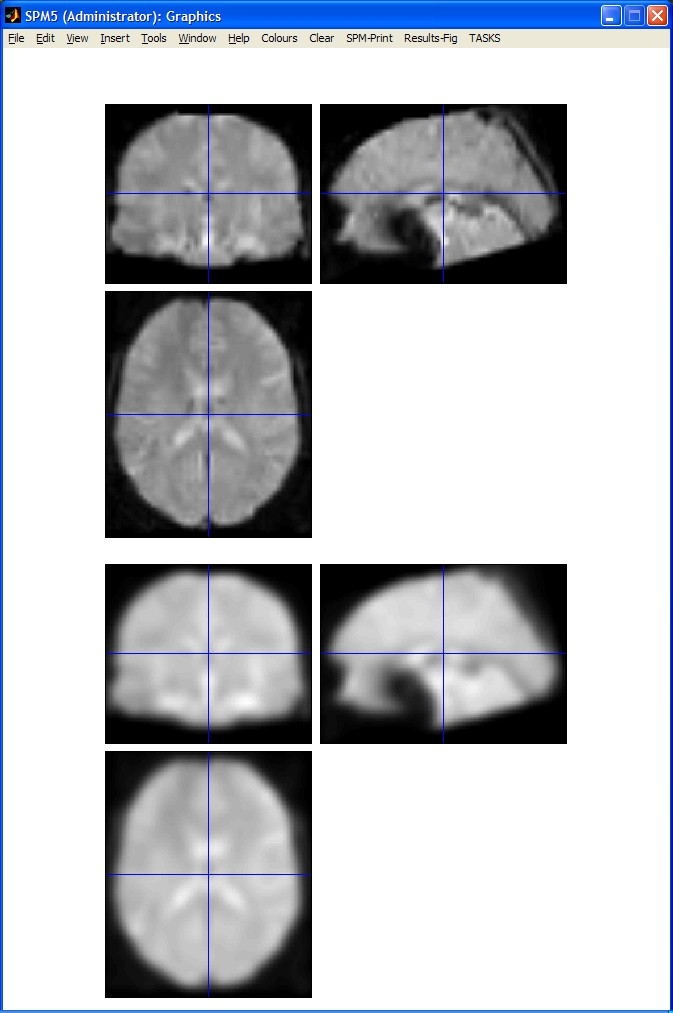
\includegraphics[width=100mm]{smooth}
\caption{\em Functional image (top) and 8mm-smoothed functional image (bottom). These images were obtained using SPM's `CheckReg' facility. \label{face_smooth}}
\end{center}
\end{figure}

\section{Modelling categorical responses}


Before setting up the design matrix we must first 
load the Stimulus Onsets Times (SOTs) and movement
parameters into matlab. SOTs are stored in the 
\verb!sots.mat! file in a 
cell array such that eg. \verb!sot{1}! contains 
stimulus onset times in TRs for event type 1, which is N1. Event-types 2,3 and 4 are N2, F1 and F2\footnote{Also included included with this data set are variables describing two event-types of no interest - the (rare) errors made by this subject on the fame-judgement task. 
We will not, however, be using these in our analyses.}.

\bi
\item{At the matlab command prompt type 'load sots'}
\item{Then type `load movepars.txt'}
\ei

Now press the `Specify 1st-level' button. This will call up the specification of a fMRI specification job in the graphics window. Then
\bi
\item{Open the fMRI model specification option}
\item{Open the `Timing paramaters' option}
\item{Highlight `Units for design' and select `Scans'}
\item{Highlight `Interscan interval' and enter 2}
\item{Highlight `Microtime resolution' and enter 24}
\item{Highlight `Microtime onset' and enter 12. These last two options make the creating of regressors commensurate with the slice-time correction we have 
applied to the data.}
\item{Highlight `Data and Design' and select `New Subject/Session'. Then open the newly created `Subject/Session' option.}
\item{Highlight `Scans' and use SPM's file selector to 
choose the 351 smoothed, normalised, slice-time corrected, realigned functional images ie  \verb!swarsM.img!. These can be selected 
easily using the \verb!^swar.*'! filter, and select all. Then press `Done'.}
\item{Highlight `Conditions' and select `New condition'}
\item{Open the newly created `Condition' option. Highlight `Name' and enter `N1'. Highlight `Onsets' and enter `sot\{1\}'. Highlight `Durations' and enter 0.}
\item{Highlight `Conditions' and select `New condition'}
\item{Open the newly created `Condition' option. Highlight `Name' and enter `N2'. Highlight `Onsets' and enter `sot\{2\}'. Highlight `Durations' and enter 0.}
\item{Highlight `Conditions' and select `New condition'}
\item{Open the newly created `Condition' option. Highlight `Name' and enter `F1'. Highlight `Onsets' and enter `sot\{3\}'. Highlight `Durations' and enter 0.}
\item{Highlight `Conditions' and select `New condition'}
\item{Open the newly created `Condition' option. Highlight `Name' and enter `F2'. Highlight `Onsets' and enter `sot\{4\}'. Highlight `Durations' and enter 0.}
\item{Highlight `Regressors', select `New Regressor', open the newly created `Regressor' option, highlight `Name' enter 'tx', highlight `Value', enter \verb!movepars(:,1)!}
\item{Highlight `Regressors', select `New Regressor', open the newly created `Regressor' option, highlight `Name' enter 'ty', highlight `Value', enter \verb!movepars(:,2)!}
\item{Highlight `Regressors', select `New Regressor', open the newly created `Regressor' option, highlight `Name' enter 'tz', highlight `Value', enter \verb!movepars(:,3)!}
\item{Highlight `Regressors', select `New Regressor', open the newly created `Regressor' option, highlight `Name' enter 'pitch', highlight `Value', enter \verb!movepars(:,4)!}
\item{Highlight `Regressors', select `New Regressor', open the newly created `Regressor' option, highlight `Name' enter 'roll', highlight `Value', enter \verb!movepars(:,5)!}
\item{Highlight `Regressors', select `New Regressor', open the newly created `Regressor' option, highlight `Name' enter 'yaw', highlight `Value', enter \verb!movepars(:,6)!}
\item{Highlight `Factorial Design', select `New Factor', open the newly created `Factor' option, highlight `Name' and enter 'Fam', highlight `Levels' and enter 2.}
\item{Highlight `Factorial Design', select `New Factor', open the newly created `Factor' option, highlight `Name' and enter 'Rep', highlight `Levels' and enter 2\footnote{The order of naming these factors is important - the factor to be specified first is the one that `changes slowest' ie. as we go through the list of conditions N1,N2,F1,F2 the factor `repetition' changes every condition and the 
factor `fame' changes every other condition. So `Fam' changes slowest and is entered first.}.}
\item{Open `Canonical HRF' under `Basis Functions'. Select `Model derivatives' and select `Time derivatives'.}
\item{Highlight `Directory' and select the \verb!DIR/designs/categorical! directory you created earlier.}
\item{Save the job as \verb!categorical_spec.mat! and press `RUN'}
\ei
SPM will then write an \verb$SPM.mat$ file to the 
\verb!DIR/designs/categorical! directory. It will also plot the design
matrix, as shown in Figure~\ref{cat_design}. 
\begin{figure}
\begin{center}
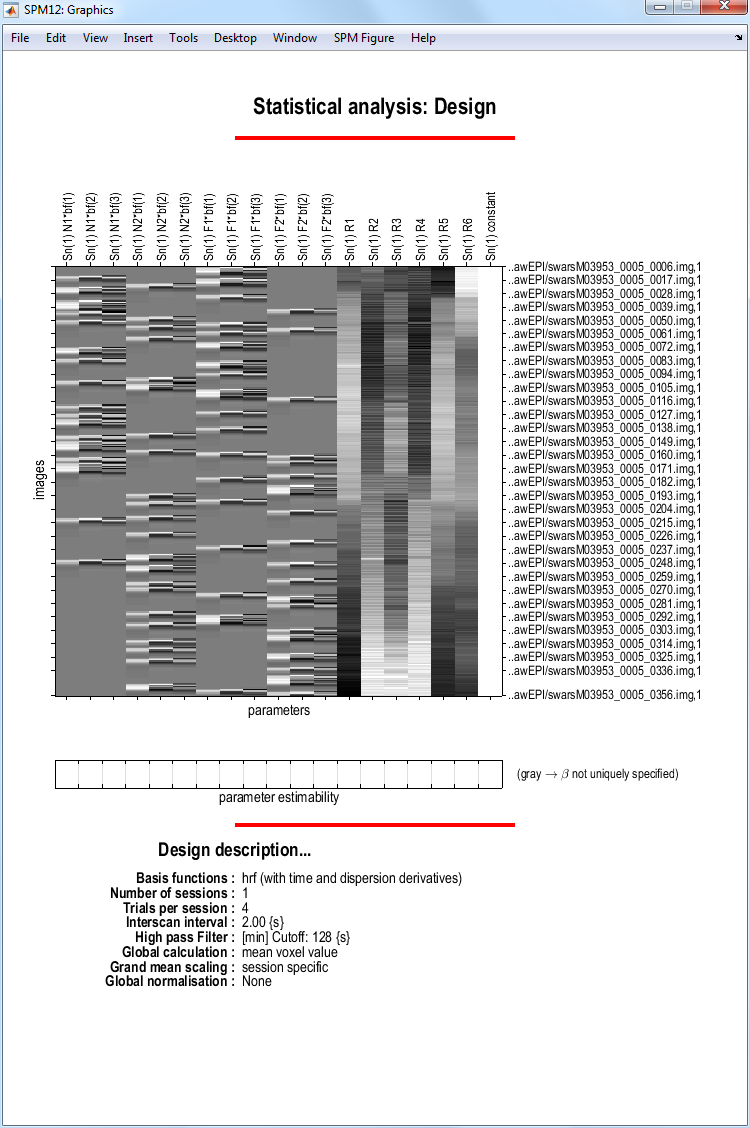
\includegraphics[width=100mm]{cat_design}
\caption{\em Design matrix. \label{cat_design}}
\end{center}
\end{figure}

At this stage it is advisable to check your model specification
using SPM's review facility which is accessed via
the `Review' button. This brings up a `design' tab on the 
interactive window clicking on which produces a pulldown
menu. If you select the first item `Design Matrix' SPM will 
produce the image shown in Figure~\ref{cat_design}. 
If you select `Explore' then `Session 1' then `N1', SPM will produce 
the plots shown in Figure~\ref{cat_explore}.
\begin{figure}
\begin{center}
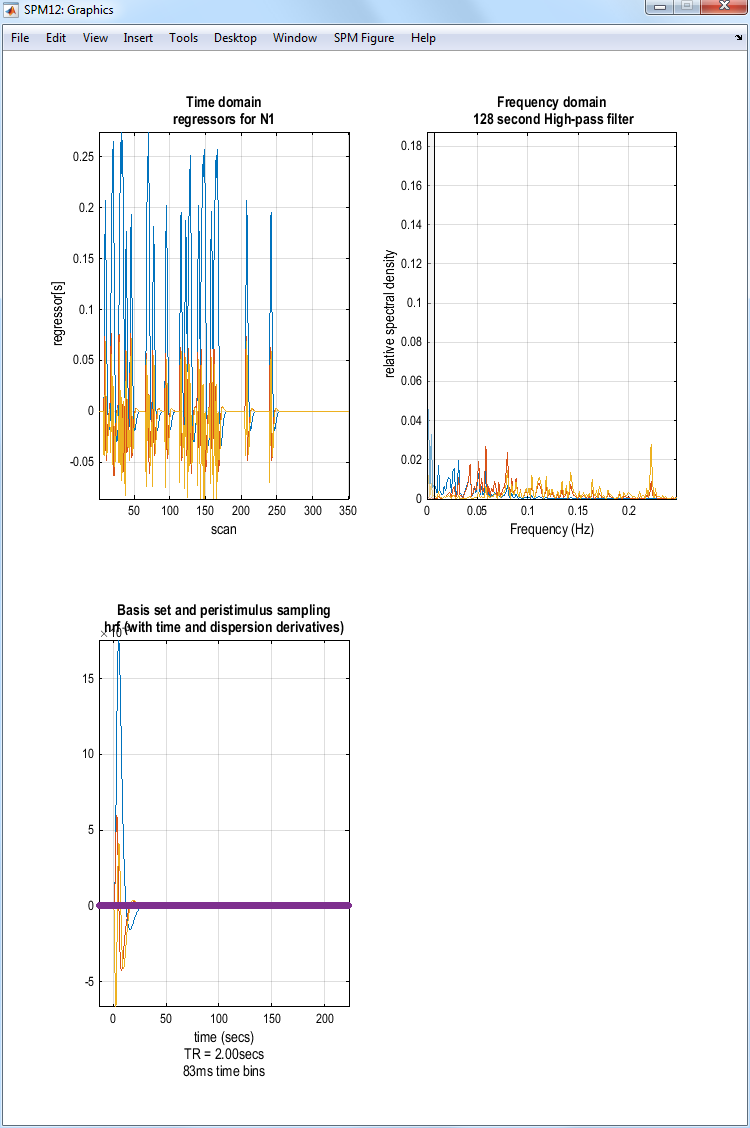
\includegraphics[width=100mm]{cat_explore}
\caption{\em Exploring the design matrix in Figure~\ref{cat_design}. This shows the time series of the `active' regressor (top left), a frequency domain plot of the active regressor (top right) and the basis function 
used to convert assumed neuronal activity into hemodynamic 
activity. In this model we used the default option - the canonical basis function. The 
frequency domain plot shows that the frequency content of the `N1' regressor is above the set
frequencies that are removed by the High Pass Filter (HPF) (these are shown in 
gray - in this model we accepted the default HPF cut-off of 128s or 0.008Hz).} \label{cat_explore}}
\end{center}
\end{figure}

\subsection{Estimate}

Press the `Estimate' button. This will call up the specification of an fMRI estimation job in the graphics window. Then
\bi
\item{Open the `fMRI model estimation' option}
\item{Highlight the `Select SPM.mat' option and then choose the SPM.mat
file saved in the \verb!DIR/designs/categorical! directory}
\item{Highlight the `Directory' option and then choose the 
\verb!DIR/classical/categorical! directory}
\item{Save the job as \verb!categorical_est.job! and press Run}
\ei
SPM will write a number of files into the selected directory including 
an \verb!SPM.mat! file.



\section{Modelling parametric responses}

In addition to analysing the data in the above "categorical" design, an alternative "parametric" design is illustrated in which repetition is viewed as a continuum. In this case, the response to each presentation of famous and non-famous faces is modulated by the time interval (lag) since the previous presentation of that face (for first presentations, this lag is infinite). 

\section{Inference for categorical design}

Press 'Results' and select the SPM.mat file from 
\verb!DIR\classical\categorical!. This will again invoke the contrast manager. Because we specified that 
our model was using a `Factorial design' a number of 
contrasts have been specified automatically, as shown 
in Figure~\ref{cat_contrasts}.
\begin{figure}
\begin{center}
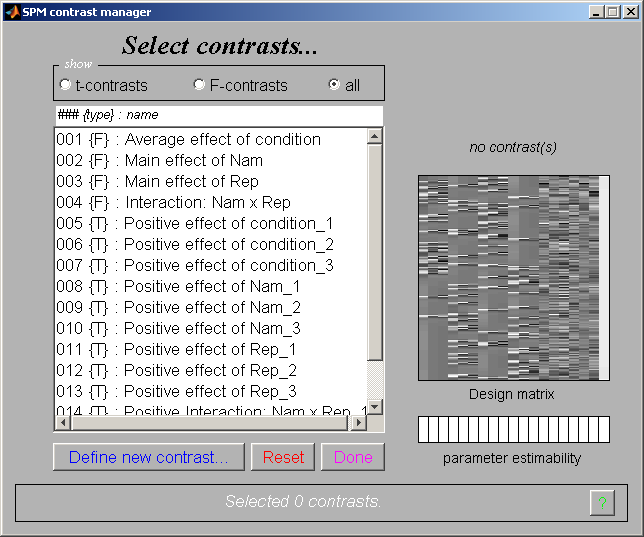
\includegraphics[width=100mm]{cat_contrasts}
\caption{\em Contrast Manager containing default contrasts for categorical design. \label{cat_contrasts}}
\end{center}
\end{figure}
To assess the main effects of viewing faces vs. baseline, select `Define new contrast' and type `Canonical HRF: Faces $>$ Baseline' (name) and `1 0 1 0 1 0 1 0' (contrast), and press `Done'.


\bi
\item{Select contrast number 5. This is a t-contrast \verb!Positive effect of condition_1! This will show 
regions where the average effect of presenting faces (condition) is significantly positive, as modelled by 
the first regressor (hence the \verb!_1!), the 
canonical HRF. Press `Done'.}
\item{\em Mask with other contrast ? [Yes/No]}
\item{Specify No.}
\item{\em Title for comparison ?}
\item{Enter `Canonical HRF: Faces > Baseline'}
\item{\em p value adjustment to control: [FWE/FDR/none]}
\item{Select FWE}
\item{\em Corrected p value(family-wise error)}
\item{Accept the default value, 0.05}
\item{\em Extent threshold \{voxels\} [0]}
\item{Accept the default value, 0}
\ei
SPM will produce a MIP.

\subsection{Statistical tables}

To get a summary of local maxima, press the `volume' button in the 
p-values section of the interactive window. This will list all clusters above the chosen level of significance as well as separate ($>$8mm apart) maxima within a cluster, with details of significance thresholds and search volume underneath, as shown in Figure~\ref{cat5_volume}
\begin{figure}
\begin{center}
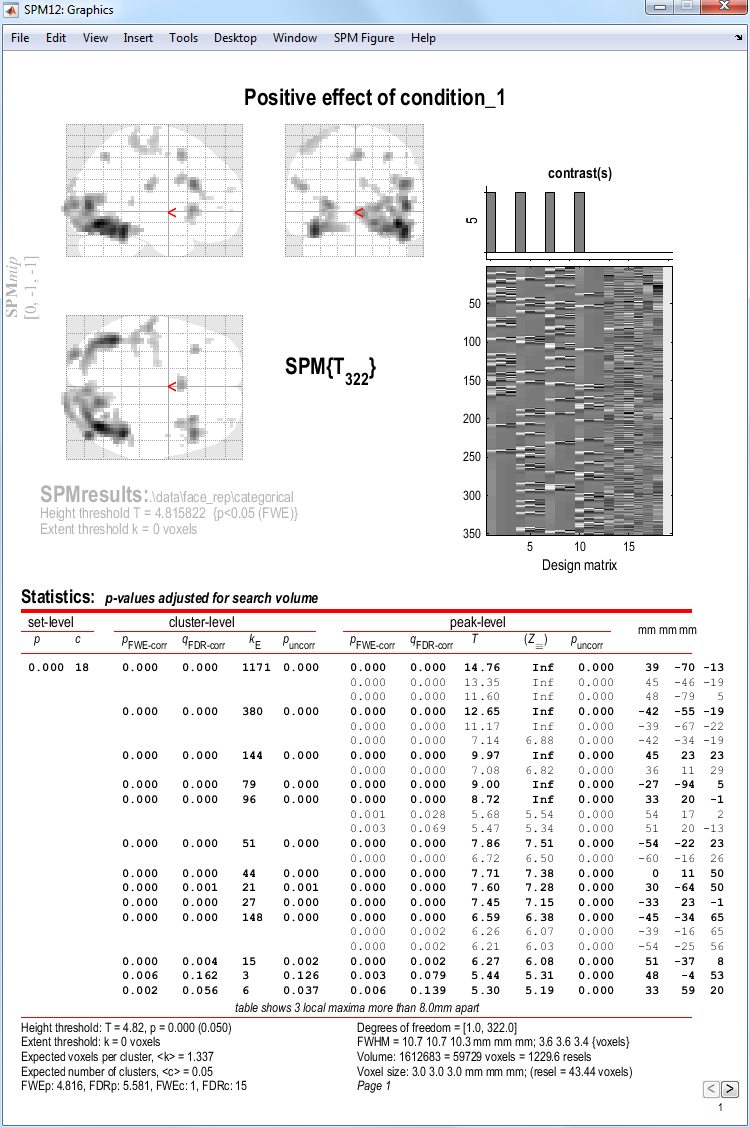
\includegraphics[width=100mm]{cat5_volume}
\caption{\em MIP and Volume table for Canonical HRF: Faces  $>$ Baseline. \label{cat5_volume} }
\end{center}
\end{figure}
The columns in volume table show, from right to left:
\bi
\item{x, y, z (mm): coordinates in Talairach space for each maximum}
\item{voxel-level: the chance (p) of finding (under the null hypothesis) a voxel with this or a greater height (T- or Z-statistic), corrected (FWE or FDR)/ uncorrected for search volume.}
\item{cluster-level: the chance (p) of finding a cluster with this many(ke) or a greater number of voxels, corrected / uncorrected for search volume}
\item{set-level: the chance (p) of finding this (c) or a greater number of clusters in the search volume}
\ei

To assess both the hrf and its temporal derivative, an F-contrast is required. 

\subsection{F-contrasts}

Press 'Results', select the SPM.mat file, and press 'F-contrast' (radio button). Next, select 'Define new contrast', specify 'hrf + temp deriv: Faces vs. Baseline' (name) and enter
'1 0 1 0 1 0 1 0
0 1 0 1 0 1 0 1 ' (contrast) and press 'Done':
 
Select the new contrast, specify 'mask with other images?' (no), specify 'name of comparison' (accept default), specify 'corrected height threshold' (yes), specify 'corrected p value' (accept default). Again, when the MIP appears, press 'Volume'.

Although the MIP of this F-contrast looks similar to the previous t-contrast, note that the present contrast shows the areas for which the mean of the parameter estimates for the canonical hrf OR its temporal derivative for the four conditions are different from zero (baseline). In other words, the F-contrast is two-sided, and tests two t-contrasts simultaneously. Also note that an F- (or t-) contrast such as 1 1 1 1 1 1 1 1, which tests whether the mean of the canonical hrf AND its temporal derivative for all conditions are different from (larger than) zero is not sensible. This is because the canonical hrf and its temporal derivative may cancel each other out while being significant in their own right. Finally, note that single F-contrasts can be regarded as $t^2$-contrasts, so that the F-contrasts 1 0 -1 0 1 0 -1 0 and -1 0 1 0 -1 0 1 0 are equivalent. 

The relative contributions of the canonical hrf and its temporal derivative at a given voxel may also be assessed using F-contrasts to estimate a reduced model, removing all confounds. Press 'Results', select the SPM.mat file, press 'F-contrast' in the contrast manager, and select 'Define new contrast'. Specify 'Effects of Real Interest' (name) and type '9:19' in the small window labelled 'columns for reduced design'. This will remove columns 9 to 19 (i.e., hrf and temporal derivative for events representing error judgements and nuisance covariates) from the design. 

Submit and select the new contrast, specify 'mask with other images?' (no), specify 'name of comparison' (accept default), specify 'corrected height threshold' (yes), specify 'corrected p value' (accept default). Again, when the MIP appears, press 'Volume'.

\subsection{Plotting parameter estimates at a voxel}

Move the cursor to e.g. the anterior right fusiform blob (the R fusiform face area) by clicking the second set of coordinates in the cluster (45 -48 -27) and press 'plot'. Select 'Contrast of parameter estimates' and select 'Effects of real interest'.

Columns 1,3,5,7 are the canonical hrfs for N1 (non-famous faces, first presentation), N2 (non-famous faces, second presentation), F1 (famous faces, 1st presentation) and F2 (famous faces, 2nd presentation), whereas columns 2,4,6,8 are the temporal derivatives. Note that the amplitude of the canonical hrfs is large compared to the temporal derivatives, suggesting that, for this region at least, the timing of the model is adequate. Also note the repetition x stimulus type interaction (the decrease from N1 to N2 is smaller than for F1 to F2).

\subsection{Masking F-contrasts}

To assess further the effects of stimulus repetition, press 'Results', select the SPM.mat file, and press 'F-contrast'. Specify e.g. 'hrf + temp deriv: 1 vs. 2' (name) and
'1 0 -1 0 1 0 -1 0
0 1 0 -1 0 1 0 -1' (contrast). Submit and select the contrast. Specify 'mask with another contrast' (yes), select the 'Canonical HRF: Faces $>$ Baseline' t-contrast, specify 'threshold for mask' (accept default of p=0.05 uncorrected), specify 'nature of mask' (inclusive), specify 'title for comparison' (accept default), specify 'corrected height threshold' (no), specify threshold (0.001). 
Again, when the MIP appears, press 'Volume'.

The MIP shows all clusters where the difference between the parameter estimates for first and second presentations for the canonical hrf OR its temporal derivative is significantly different from zero AND the canonical hrf for all four conditions is significantly larger than zero. Note that although the mask does not alter the threshold for the target contrast, the combined probability for a voxel to appear in the masked contrast is in the order of 0.05 x 0.001 uncorrected due to the orthogonality of the contrasts. 

\subsection{Plotting event-related responses}

To plot repetition suppression effects for the R fusiform region, select the third cluster from the top (by clicking 48 60 -15; slightly more posterior to that identified above) and press 'plot'.
Select  'event-related responses'.
\bi
\item{\em Which trials or conditions (1 to 6)}
\item{Specify `1:4'}
\item{\em Plot in terms of ...}
\item{Select fitted response and PSTH}
\ei
To adjust the scale of the x-axis (time), press 'attrib' from the plot controls panel.
Select Xlim, and change the default (-4 32) to '0 10'.

Note the signal decrease between first and second presentations of both famous and non-famous faces.
Other options from the plot controls panel:
\bi
\item{Hold: allows overlaying of plots}
\item{Grid: toggles between grid on/off}
\item{Box: toggles between axes/box}
\item{Text: allows editing of title and/or axis labels.}
\ei

\subsection{F-contrasts for testing effects of movement}

To assess movement-related activation, press 'Results', select the SPM.mat file, and select 'F-contrast' in the Contrast Manager. Specify e.g. 'Movement-related activation' (name) and either {\sf [zeros(6,12),eye(6)]}
in the 'contrasts weights matrix' window, or '1:12 19' in the 'columns for reduced design' window. 
 
Submit and select the contrast, specify 'mask with other contrasts?' (no), 'title for comparison' (accept default), 'corrected height threshold' (yes), and 'corrected p-value' (accept default). When the MIP appears, press `Volume'.

The table displays all clusters where signal changes correlated with any of the six movement parameters are significantly different from zero. Note the large edge effects, which, however, are not apparent in the fusiform regions.

\subsection{Parametric modulation}

Finally, consider the effects of the interval between first and second presentations of famous and non-famous faces. For this purpose, an alternative statistical model needs to be estimated, with four trial types. (1) First and second presentation of a non-famous face (N1 and N2 collapsed). (2) First and second presentation of a famous face (F1 and F2 collapsed). (3) Errors in judging non-famous faces. (4) Errors in judging famous faces. These are modelled with the canonical hrf alone, with two parametric (exponential) modulations added for second presentations of non-famous and famous faces. See the README.txt for details of design specification.

After completion of model estimation, press `Results' and select the SPM.mat file. When the Contrast Manager appears, define an F-contrast `Effect of Lag (on canonical N+F)' (name) and `0 1 0 1', and a t-contrast `Canonical: Faces $>$ Baseline' (name) and `1 0 1 0'. Select the F-contrast, specify `mask with other contrasts' (yes), select `Canonical: Faces $>$ Baseline', specify `uncorrected mask p-value' (accept default), `nature of mask (inclusive), `title for comparison' (accept default), `corrected height threshold' (no), and `corrected p-value' (accept default). When the MIP appears, press `Volume'.

The table displays all clusters where the exponential change in activation between first and second presentations for famous OR non-famous faces for the canonical hrf is significantly different from zero AND the canonical hrf for the first two conditions is significantly larger than zero (baseline). We can now 
plot these parametric effects at particular voxels.

\subsection{Plotting parametric responses}

To plot these parametric effects, select the R fusiform region (45 -60 -18, similar to the region identified in the previous categorical analysis for repetition effects), and press 'plot'. Select 'Plots of parametric responses' and select 'F' (or 'N').  Note that the 'attrib' option does not allow adjustment of the scale of the Z-axis; therefore, to change the scale for all axes, type e.g. 'figure (1), axis ([0 30 0 100 0 1])' in the Matlab window.

Note that these repetition effects are transient (decrease with increasing intervals between first and second presentations), especially for famous faces.

\end{document}